\documentclass[a4paper,12pt]{article}
\usepackage[a4paper,top=1.3cm,bottom=2cm,left=1.5cm,right=1.5cm,marginparwidth=0.75cm]{geometry}
\usepackage{cmap}
\usepackage{mathtext}
\usepackage[T2A]{fontenc}
\usepackage[utf8]{inputenc}
\usepackage[english,russian]{babel}
\usepackage{siunitx}
\usepackage{enumitem}
\usepackage{placeins}

\usepackage{graphicx}

\usepackage{wrapfig}
\usepackage{tabularx}
\usepackage{multirow}

\usepackage{hyperref}
\usepackage[rgb]{xcolor}
\hypersetup{
colorlinks=true,urlcolor=blue
}
\usepackage{amsmath,amsfonts,amssymb,amsthm,mathtools}
\usepackage{icomma}
\mathtoolsset{showonlyrefs=false}
\usepackage{euscript}
\usepackage{mathrsfs}
\DeclareMathOperator{\sgn}{\mathop{sgn}}
\newcommand*{\hm}[1]{#1\nobreak\discretionary{}
{\hbox{$\mathsurround=0pt #1$}}{}}

%%% Заголовок
\author{Макаров Лев Евгеньевич}
\title{Лабораторная работа №3.5.1

Изучение плазмы газового разряда в неоне
}
\date{\today}

%%% Заголовок
\author{Макаров Лев Евгеньевич}
\title{Лабораторная работа №3.2.6

Изучение гальванометра
}
\date{\today}

\begin{document}

\begin{titlepage}
	\begin{center}
		{\large МОСКОВСКИЙ ФИЗИКО-ТЕХНИЧЕСКИЙ ИНСТИТУТ (НАЦИОНАЛЬНЫЙ ИССЛЕДОВАТЕЛЬСКИЙ УНИВЕРСИТЕТ)}
	\end{center}
	\begin{center}
		{\large Физтех-школа фотоники, электроники и молекулярной физики}
	\end{center}
	
	
	\vspace{4.5cm}
	{\huge
		\begin{center}
			{\bf Отчёт о выполнении лабораторной работы 3.2.6}\\
			Изучение гальванометра
		\end{center}
	}
	\vspace{2cm}
	\begin{flushright}
		{\LARGE Автор:\\ Макаров Лев Евгеньевич \\
			\vspace{0.2cm}
			Б04-306}
	\end{flushright}
	\vspace{8cm}
	\begin{center}
		Долгопрудный 2024
	\end{center}
\end{titlepage}

\section{Введение}

\textbf{Цель работы:} 
\begin{enumerate}
	\item Изучение работы высокочувствительного зеркального гальванометра магнитоэлектрической системы в режимах измерения постоянного тока и электрического заряда.
\end{enumerate}

\textbf{В работе используются:} 
\begin{itemize}
    \item зеркальный гальванометр с осветителем и шкалой
    \item источник постоянного напряжения
    \item делитель напряжения
    \item магазин сопротивлений
    \item эталонный конденсатор
    \item вольтметр
    \item переключатель
    \item ключи
    \item линейка
\end{itemize}
\medskip

\section{Теоретические сведения}

\begin{wrapfigure}{l}{0.35\linewidth} 
    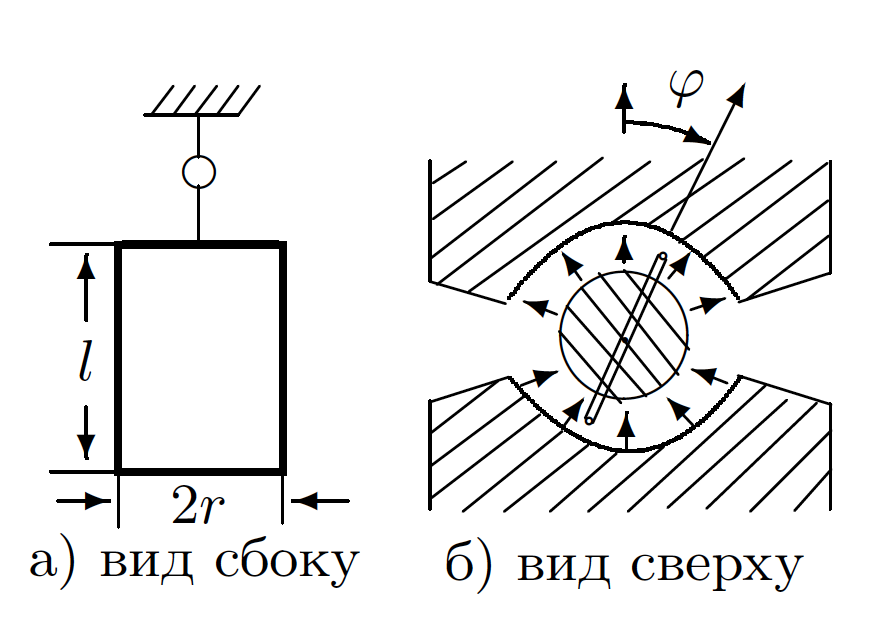
\includegraphics[width=6cm]{ramka}
    \caption{Рамка}
    \label{}
\end{wrapfigure}

Главной частью высокочувствительного гальванометра магнитоэлектрической системы является подвешенная на вертикальной нити рамка, помещённая в поле постоянного магнита (рис. 1). Вырез цилиндрической формы в полюсах магнита и ферромагнитный цилиндр на оси системы делают поле в зазоре радиальным. Скреплённое с рамкой зеркальце служит для измерения угла поворота рамки. Магнит и подвижная система заключены в защитный кожух.

Запишем основное уравнение колебаний рамки:

\begin{equation}\label{main}
\ddot{\phi} + 2\gamma\dot{\phi }+ \omega_0^2\phi = K I
\end{equation}
	
где введены обозначения: $ 2\gamma = \dfrac{(BSN)^2}{JR_\Sigma} $, $ \omega_0^2 = \dfrac{D}{J}, K = \dfrac{BSN}{J} $. Эти величины выражены через параметры установки: $ B $ --- магнитное поле, в которое помещена рамка, $ I  = \dfrac{\varepsilon}{R_\Sigma}$ --- ток, текущий через рамку, $ R_\Sigma $ --- сопротивление рамки и цепи, $ N $ --- число витков рамки, $ S $ --- площадь витка рамки, $ J $ --- момент инерции системы, $ D $ --- модуль кручения нити.

\subsection{Стационарный режим}
Если через рамку пропускать постоянный ток (достаточно дол-
го, чтобы затухли колебания подвижной системы), то в уравнении \eqref{main} можно положить $ \ddot{\phi} = \dot{\phi } = 0 $, и угол поворота определится формулой

\begin{equation}\label{C1}
\phi = \dfrac{I}{C_1}, \qquad C_I = \dfrac{D}{BSN} = \dfrac{I}{\phi}
\end{equation}

где $ C_I $ --- динамическая постоянная гальванометра.

\subsection{Свободные колебания}

При отсутствии внешнего источника тока, мы получаем, что левая часть уравнения \eqref{main} равна нулю. Это обычное уравнение колебаний, решение и свойства которого рассматривались в курсе механики и прошлой работе 3.2.4., не будем останавливаться на нем подробно, напомним лишь, что в зависимости параметра $ \gamma $ у нас есть колебательный режим, критический режим и случай переуспокоенного гальванометра, причем в последних двух случаях движение апериодическое. 

\subsection{Баллистический режим}

Период свободных колебаний баллистического гальванометра благодаря искусственному увеличению момента инерции рамки оказывается очень большим (порядка десяти секунд). Если пропустить через рамку короткий импульс тока, то можно считать, что весь ток успевает пройти при неотклоненном положении рамки. Рамка, однако, при этом получает толчок, в результате которого возникает движение, описываемое уравнением свободных колебаний при начальных условиях $ \phi(t) = 0, \dot{\phi }(0) = \dot{\phi }_0 $.

Для вычисления скорости $ \dot{\phi }_0 $, полученной в результате толчка, умножим уравнение \eqref{main} на $ dt $ и проинтегрируем его по времени от 0 до момента окончания токового импульса $ \tau $. Пренебрегая малыми вторым и третьим членом в левой части, получаем,

\begin{equation}\label{q}
\int\limits_0^\tau \ddot{\phi}dt = K 	\int\limits_0^\tau I dt \te \dot{\phi }(\tau) = Kq
\end{equation}

где $ q $ --- полный электрический заряд, прошедший через рамку за время импульса. При этом мы пренебрегаем зарядом индукционного тока.


Величина $ C_Q = \dfrac{q}{\phi_{max}}$ называется баллистической постоянной гальванометра. Баллистическая постоянная наряду с динамической является важнейшей характеристикой гальванометра, но в отличие от динамической она существенно зависит от режима работы гальванометра (от сопротивления цепи).

Расчёт показывает, что максимальный отброс достигается при полном
отсутствии затухания (тормозящий индукционный ток отсутствует при
обрыве в цепи):

\begin{equation}\label{}
\phi_{max \; св} = \dfrac{\dot{\phi }(\tau) }{\omega_0} = \dfrac{Kq}{\omega_0}
\end{equation}

В этом случае, однако, возникшие в результате отброса колебания рам-
ки не будут успокаиваться, и прибор не скоро сможет быть использован
для повторных измерений.

Обычно удобнее всего работать в режиме, близком к критическому:

\begin{equation}\label{}
\phi_{max \; кр} = \dfrac{Kq}{\omega_0 e}
\end{equation}

Таким образом, в критическом режиме максимальное отклонение зайчика в $ e $ раз меньше, чем в режиме свободных колебаний. Отсюда, в частности,  следует, что отношение баллистических постоянных

\begin{equation}\label{}
\dfrac{C_{Q \; кр}}{C_{Q \; св}} = e
\end{equation}

\section{Экспериментальная установка}

\subsection{Стационарный ток}

В режиме стационарного тока можно легко вычислить ток по формуле 

\begin{equation}\label{I}
I = U_0 \dfrac{R_1}{R_2} \dfrac{1}{R + R_0}
\end{equation}

Координата $ x $ зайчика связана с углом $ \phi $ простым соотношением $ x = a\tg 2\phi $, и при малых $ \phi  =  \dfrac{x}{2a}$, где $ a $ --- расстояние от шкалы до зеркальца. 

Отсюда из \eqref{C1} получаем:

\begin{equation}\label{C1exp}
C_I = \dfrac{2aI}{x}
\end{equation}

\begin{wrapfigure}{l}{0.65\linewidth} 
    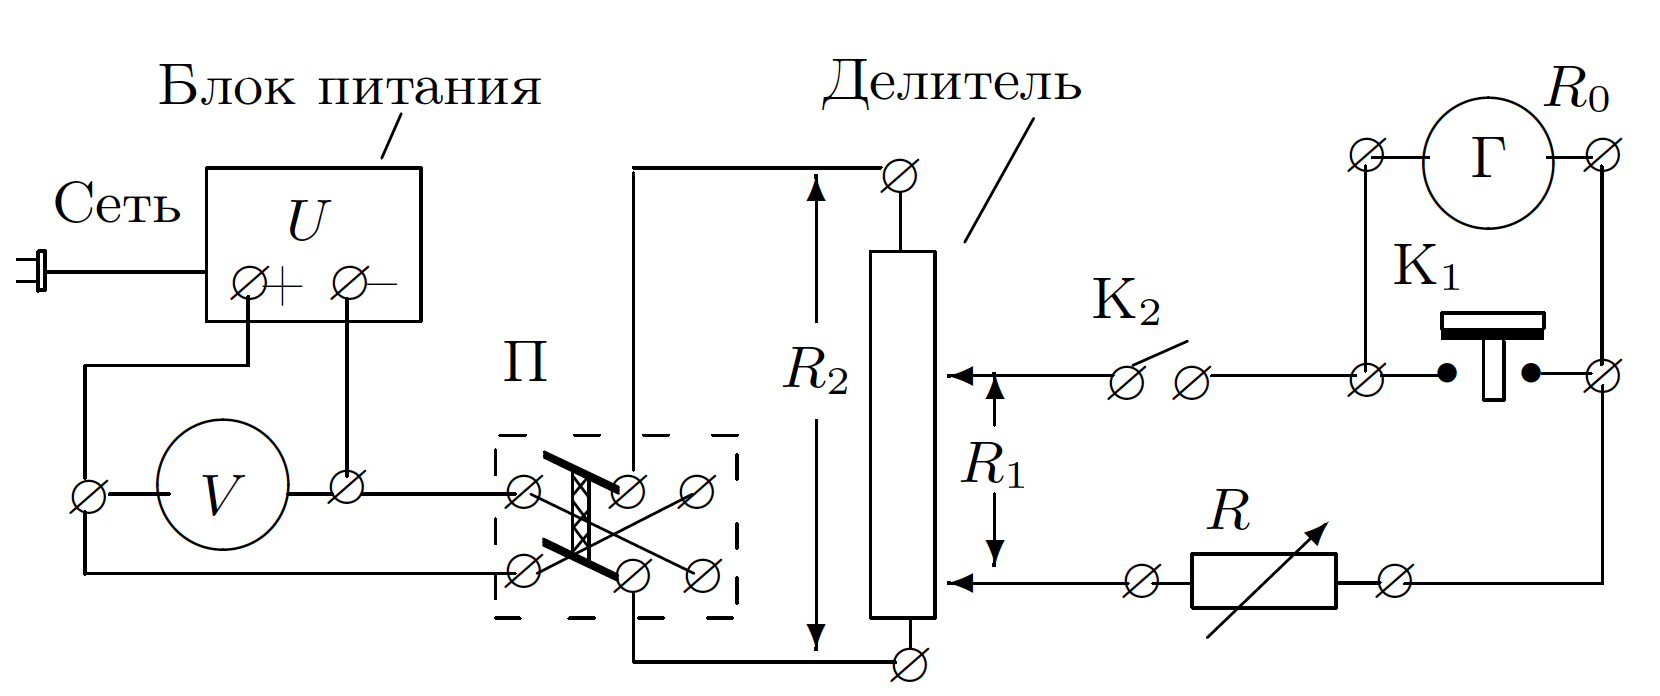
\includegraphics[width=8cm]{scheme1}
    \caption{Схема установки для первой и второй частей работы}
    \label{chain1}
\end{wrapfigure}

\subsection{Критический режим и свободные колебания}

Логарифмический декремент затухания определяется экспериментально по формуле

\begin{equation}\label{Theta}
    \Theta =  \gamma T =  \ln \dfrac{x_k}{x_{k+n}}
\end{equation}

При этом мы можем 
выразить декремент как

\begin{equation}\label{}
    \Theta =  \gamma T =  \dfrac{2\pi\gamma}{\sqrt{\omega_0^2 - \gamma^2}} = \dfrac{2\pi R_3}{\sqrt{(R + R_0)^2 - R_3^2}}
\end{equation}

где $ R_3 = R_{кр} + R_0 $. Отсюда нетрудно получить формулу: 

\begin{equation}\label{}
\dfrac{4\pi^2}{\Theta^2} = \dfrac{(R_0 + R)^2}{(R_0 + R_{кр})^2} - 1
\end{equation}

Для расчета $ R_{кр} $ будем использовать следующую формулу:

\begin{equation}\label{Rkr}
R_\text{кр} = \dfrac{R + R_0}{1 + \frac{4\pi^2}{\Theta^2}} - R_0 = const
\end{equation}
 
 Таким образом, отношение $ f(R) $ и $ F(\Theta) $ из физического смысла должно быть постоянным. 
 
 \subsection{Баллистический режим}
 \begin{wrapfigure}{l}{0.65\linewidth} 
    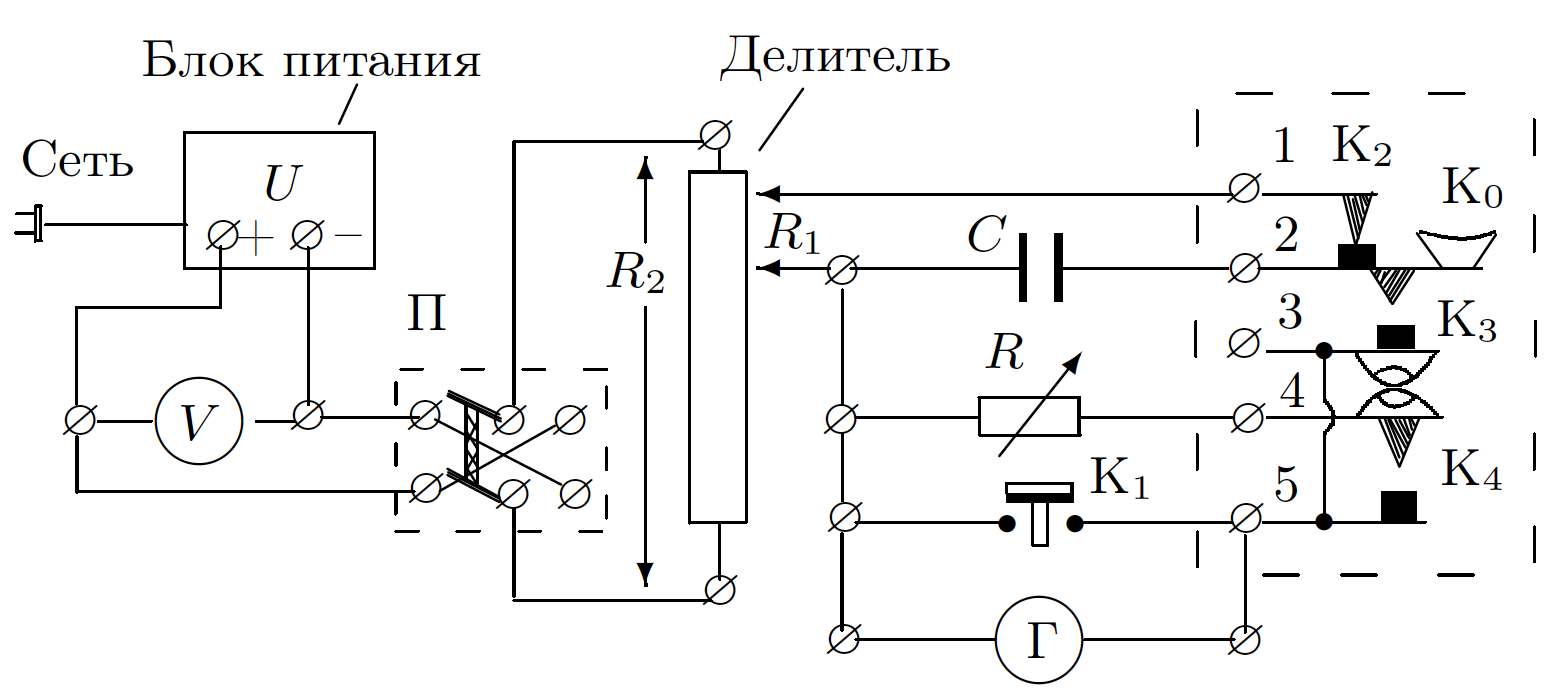
\includegraphics[width=10cm]{scheme2}
    \caption{Схема установки для третей части работы}
    \label{chain2}
 \end{wrapfigure}
 
 Заряд конденсатора $ C $ равен 
 
 \begin{equation}\label{}
 q = U_C C = C \dfrac{R_1}{R_2}U_0
 \end{equation}
 
 Из решения уравнения колебаний и формулы декремента следует формула 
 
 \begin{equation}\label{}
 l_0 = l_1 e^{\Theta/4}
 \end{equation}
 
 При сопротивлении, равном критическому, баллистическая постоянная будет определяться
 
 \begin{equation}
 C_{Q кр} = \dfrac{q}{\phi_{max \; кр}} = 2a\dfrac{R_1}{R_2}\dfrac{U_0C}{l_{max \; кр}}
 \label{C}
 \end{equation}

\section{Результаты измерений и обработка данных}

\subsection*{I. Подготовка приборов к работе}

\begin{enumerate}
    \item Настроим осветитель гальванометра так, чтобы на шкале появилась четкая вертикальная риска и полдожение равновесия совпадало с нулем на шкале.
    \item Установим делитель в положение $R_1/R_2 = 1/2000$, а сопротивление магазина $R = 50$ кОм.
    \item Соберем схему согласно рис. \ref{chain1}.
    \item При разомкнутых ключах К2 и К3 включим в сеть блок питания и замкнем ключ К3.
    \item Включим осветитель гальванометра
    \item Замкнем ключ К2 и подберем сопротивление магазина, при котором зайчик отклоняется почти на всю шкалу, $R = 12$ кОм.
\end{enumerate}

\subsection*{II. Определение динамической постоянной}

\begin{enumerate}[resume]
    \item Измерим зависимость отклонения зайчика от сопротивления, увеличивая сопротивление. $U_0 = 2$ В, $R_1/R_2 = 1/2000$, $R_0 = 475$ Ом, $R_2 = 10$ кОм. Результаты измерений запишем в таблицу \ref{table:1}.
\end{enumerate}

\FloatBarrier
\begin{table}[!h]
    \centering
    \caption{Зависимость $I(x)$}
    \begin{tabular}{|l|l|l|l|}
        \hline
        $N$  & $R$, кОм & $x$, см & $I$, мкА \\ \hline
        1  & 12     & 21.4  & 2.053  \\ \hline
        2  & 14     & 18.5  & 2.045  \\ \hline
        3  & 16     & 16.3  & 2.037  \\ \hline
        4  & 18     & 14.6  & 2.028  \\ \hline
        5  & 20     & 13.3  & 2.020  \\ \hline
        6  & 22     & 12.1  & 2.012  \\ \hline
        7  & 24     & 11.2  & 2.004  \\ \hline
        8  & 26     & 10.3  & 1.996  \\ \hline
        9  & 28     & 9.6   & 1.988  \\ \hline
        10 & 30     & 9.0   & 1.980  \\ \hline
    \end{tabular}
    \label{table:1}
\end{table}

\subsection*{III. Измерение критического сопротивления}

\begin{enumerate}[resume]
    \item Установим значение $R$, при котором зайчик отклоняется почти на всю шкалу.
    \item Разомкнем ключ К2. Измерим два последовательных колебания в одну сторону и рассчитаем логарифмический декремент затухания $\theta_0$:
\end{enumerate}

\begin{equation*}
    \theta_0 = \ln {\frac{x_1}{x_2}} = \ln {\frac{21.3}{17.0}} \approx 0.23
\end{equation*}

\begin{enumerate}[resume]
    \item Измерим период свободных колебаний $T_0$
\end{enumerate}

\begin{equation*}
    T_n = 46.05 \ \text{с}, n = 9 \implies T_0 = \frac{T_n}{n} \approx 5.12 \ \text{с}
\end{equation*}

\begin{enumerate}[resume]
    \item Замкнем ключ К2 и разомкнем ключ К3. Колебания затухают быстрее, так как тормозящий ток увеличился с уменьшением сопротивления.
    \item Подберем наибольшее сопротивление $R$, при котором при размыкании ключа К3зайчик не переходит за нулевое значение, оно близко к критическому
\end{enumerate}

\begin{equation*}
    R_\text{кр} \approx 7.7 \ \text{кОм}
\end{equation*}

\begin{enumerate}[resume]
    \item Установим сопротивление $R \approx 3R_\text{кр} \approx 23$ кОм. Подберем делитель так, чтобы зайчик отклонялся почти на всю шкалу. Измерим два последовательных затухания и посчитаем логарифмический декремент затухания, а также $R_\text{кр}$.
    \item Повторим измерения предыдущего пункта для нескольких значений $R$ и результаты измерений запишем в таблицу \ref{table:2}.
\end{enumerate}

\FloatBarrier
\begin{table}[!h]
    \centering
    \caption{Измерение критического сопротивления}
    \begin{tabular}{|l|l|l|l|l|l|}
        \hline
        $N$  & $R$, кОм & $x_1$, см   & $x_2$, см  & $\theta$ & $R_\text{кр}$, Ом \\ \hline
        1  & 23     & 20.7 & 2.9 & 1.97                  & 1617  \\ \hline
        2  & 28     & 17.1 & 3.3 & 1.65                  & 1329  \\ \hline
        3  & 32     & 15.1 & 3.5 & 1.46                  & 1207  \\ \hline
        4  & 37     & 24.6 & 6.6 & 1.32                  & 1096  \\ \hline
        5  & 42     & 21.8 & 6.7 & 1.18                  & 957   \\ \hline
        6  & 46     & 19.9 & 6.6 & 1.10                  & 922   \\ \hline
        7  & 54     & 17.1 & 6.6 & 0.95                  & 745   \\ \hline
        8  & 62     & 24   & 9.2 & 0.96                  & 938   \\ \hline
        9  & 69     & 21.7 & 9.6 & 0.82                  & 681   \\ \hline
        10 & 77     & 19.5 & 9.4 & 0.73                  & 556   \\ \hline
    \end{tabular}
    \label{table:2}
\end{table}

\subsection*{IV. Баллистический режим}

\begin{enumerate}[resume]
    \item Соберем схему согласно рис. \ref{chain2}. Установим сопротивление $R = 50$ кОм.
    \item Разомкнем цепь $R$ и подберем делитель так, чтобы при замыкании ключа К0 первый отброс соответствовал отклонению почти на всю шкалу. $R_1/R_2 = 1/70$.
    \item Подключим магазин $R$. Получим зависимость величины первого отброса от $R$. Измерять будем, пока первый отброс не уменьшиться в 4 раза, чтобы сохранялся критический режим. Результаты измерений запишем в таблицу \ref{table:3}.
\end{enumerate}

\FloatBarrier
\begin{table}[!h]
    \centering
    \caption{Зависимость максимального отброса от $R$}
    \begin{tabular}{|l|l|l|}
        \hline
         $N$ & $R$, кОм  & $x_{max}$, см \\ \hline
        1  & 50 & 13.5 \\ \hline
        2  & 45 & 12.9 \\ \hline
        3  & 40 & 13.4 \\ \hline
        4  & 35 & 12.4 \\ \hline
        5  & 30 & 12.6 \\ \hline
        6  & 25 & 11.5 \\ \hline
        7  & 20 & 11.7 \\ \hline
        8  & 15 & 10.5 \\ \hline
        9  & 10 & 9    \\ \hline
        10 & 5  & 6.7  \\ \hline
        11 & 4  & 5.8  \\ \hline
        12 & 3  & 5.2  \\ \hline
        13 & 2  & 4.3  \\ \hline
        14 & 1  & 3.2  \\ \hline
    \end{tabular}
    \label{table:3}
\end{table}
\FloatBarrier

\begin{enumerate}[resume]
    \item Запишем положение делителя $R_1/R_2 = 1/70$ и значение емкости $C = 2$ мкФ. Измерим расстояние от шкалы до гальванометра $a = 140$ см.
    \item Разберем схему.
\end{enumerate}

\subsection*{V. Обработка результатов}

\begin{enumerate}[resume]
    \item Построим график зависимости $I(x)$ на рис. \ref{graph:1}
\end{enumerate}

\FloatBarrier
\begin{figure}[!ht]
    \centering
	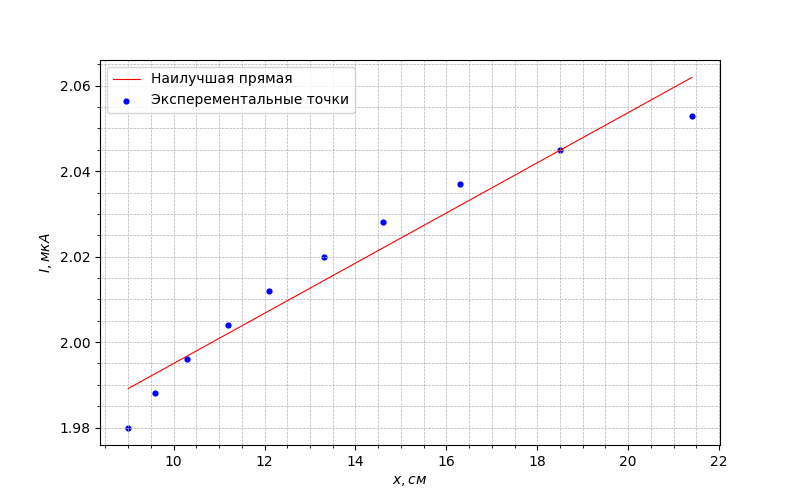
\includegraphics[width=0.9\textwidth]{graph-1.png}
	\caption{\textit{График зависимости $I(x)$}}
	\label{graph:1}
\end{figure}
\FloatBarrier

Как видно из графика шкала не является линейной.

\begin{equation*}
    k = (0.0059 \pm 0.0005) \ \text{мкА}/\text{см} \implies C_l \approx 1.65 \ \text{мкА}
\end{equation*}

\begin{enumerate}[resume]
    \item Логарифмический декремент затухания для разомкнутого гальванометра
\end{enumerate}

\begin{equation*}
    \theta_0 = 0.23
\end{equation*}

\begin{enumerate}[resume]
    \item Рассчитаем значения декрементов затухания $\theta$ для каждого $R$ и определим значение $R_\text{кр}$. Результаты в таблице \ref{table:2}.
    \item Построим график зависимости $x_{max} = f(R + R_0)$ на рис. \ref{graph:2}.
\end{enumerate}

\FloatBarrier
\begin{figure}[!ht]
    \centering
	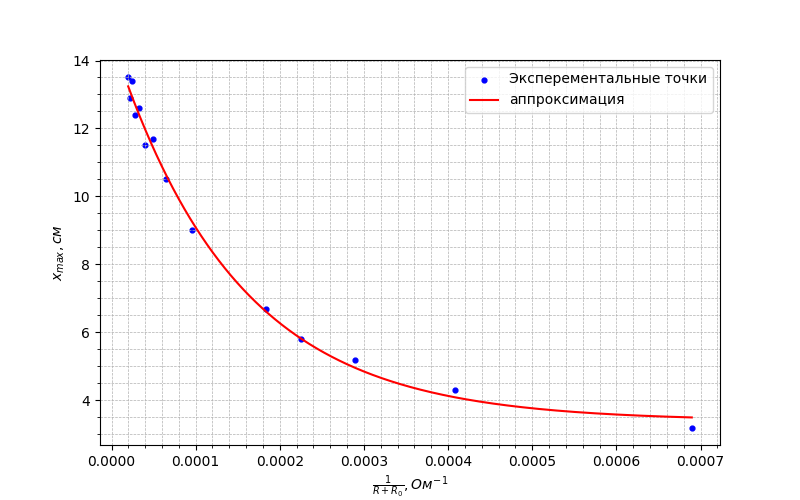
\includegraphics[width=0.9\textwidth]{graph-2.png}
	\caption{\textit{График зависимости $x_{max} = f(R + R_0)$}}
	\label{graph:2}
\end{figure}
\FloatBarrier

\begin{enumerate}[resume]
    \item Усредненное значение $R_\text{кр}$ из таблицы приблизительно совпадает с подобранным.
\end{enumerate}

Значение $l_e = l_0 e^{\theta_0/4} \approx 14.4$ см. Отсюда найдем соотвествующую точку на графике и рассчитаем $R_\text{кр} = 5.26$ кОм.

\begin{enumerate}[resume]
    \item Рассчитаем баллистическую постоянную в критическом режиме.
\end{enumerate}

\begin{equation*}
    C_q = 2a \frac{R_1}{R_2} \frac{U_0 C}{l_e} \approx 1.7 \cdot 10^{-6} \ \text{Кл}
\end{equation*}

\begin{enumerate}[resume]
    \item Сравним время релаксации и период свободных колебаний в гальванометре.
\end{enumerate}

\begin{equation*}
    \tau = R_0 C \approx 1 \ \text{мс} << T_0
\end{equation*}


\end{document}